\chapter{Introducción específica} % Main chapter title

\label{Chapter2}

%----------------------------------------------------------------------------------------
%	SECTION 1
%----------------------------------------------------------------------------------------
%Todos los capítulos deben comenzar con un breve párrafo introductorio que indique cuál es el contenido que se encontrará al leerlo.  La redacción sobre el contenido de la memoria debe hacerse en presente y todo lo referido al proyecto en pasado, siempre de modo impersonal.
En este capítulo se presentan las bases teóricas que sustentan el trabajo realizado. Se describen distintas soluciones a cada una de las partes del sistema.

\section{Descripción de tecnologías web para IoT}
\label{sec:Descripción de tecnologías web para IoT}


Los sistemas web utilizan (en su mayoría) una arquitectura cliente/servidor en donde se subdivide las tareas a desarrollar en dos partes. El cliente solicita una acción y el servidor la ejecuta. Las acciones pueden ser obtener información para mostrar en una pantalla, modificar un valor en una base de datos, obtener información para reproducir un sonido o un video, etc. En la programación web, se suele dividir el modelo en 2 partes: \textit{ backend} y \textit{frontend} .  

\subsection{ Breve introduccion a tecnologías de backend}
El \textit{backend}  generalmente se encarga de almacenar y gestionar la información \citep{ARTICLE:4}. En el contexto de este trabajo, el \textit{backend} se comunica con los clientes utilizando 2 protocolos: \textit{Message Queuing Telemetry Transport} (en adelante MQTT )  y HTTP. El primero se utilizó para interactuar con los clientes móviles y el segundo se utilizó para brindar los servicios a la página web de configuración.

El protocolo MQTT \citep{ WEBSITE:5} se ha probado como un protocolo confiable, altamente eficiente y ampliamente utilizado en sistemas IoT \citep{ARTICLE:2}.

MQTT es un protocolo open source simple, liviano y orientado a dispositivos con pocos recursos y baja velocidad de transmisión. Está basado en la pila TCP/IP(del ingles \textit{Transmission Control Protocol/Internet Protocol}, Protocolo de control de transmisión /Protocolo de Internet ), se implementa en la capa de aplicación y utiliza mensajeria bajo el patrón de publicación/subscripción. Las ventajas que provee es la posibilidad de agregar accesorios rápidamente con bajo costo de software, hardware e implementación \citep{ARTICLE:2}.

En la referencia \citep{ARTICLE:2} se realiza un estudio en profundidad del desempeño de varios protocolos de IoT: MQTT, CoAP (\textit{Constrained Application Protocol, Protocolo de Aplicaciones Restringido}), AMQP(\textit{Advanced Message Queuing Protocol}, Protocolo de Encolamiento de Mensajes Avanzado ) y HTTP (\textit{Hypertext Transfer Protocol}, Protocolo de Transferencia de Hipertexto). Se menciona que MQTT es ampliamente utilizado pero muy poco estandarizado en comparación con los demas, y se resalta el hecho que tiene limitaciones en lo referido a seguridad.

En las subcciones \ref{sec: Introducción a las bases de datos},\ref{sec:Docker},\ref{subsec:Docker-compose},\ref{subsec: Node} se explicará el funcionamiento del backend.
\subsection{Breve introduccion a tecnologías frontend}
El \textit{frontend} es la parte del programa o del dispositivo con la que interactua el usuario. Son tecnologías que se ejecutan en un navegador o en una aplicación de telefono celular (también llamado telefono inteligente, o \textit{smartphone}). El equipo que desarrolla el \textit{frontend} consiste en programadores diseñadores UX/UI (del ingles \textit{User Experience / User Iterface}, Experiencia de Usuario/Interfaz de Usuario) y diseñadores gráficos. Las más conocidas tecnologías que se utilizan son: el lenguaje de programación Javascript, HTML (\textit{HyperText Markup Language}, Lenguaje de Marcas de Hipertexto) y CSS (\textit{Cascading Style Sheets}, Hojas de Estilo en Cascada) \citep{ARTICLE:4}. Si se desea profundizar en estas tecnologías, existen muchos sitios web donde se ofrecen referencias de las mismas (ver, por ejemplo: \citep{WEBSITE:13}).  

En los últimos años, se busca facilitar el diseño de  \textit{frontend} mediante librerías como React \citep{WEBSITE:14},  JQuery \citep{WEBSITE:17} o Frameworks como ser Vue \citep{WEBSITE:15}, Angular \citep{WEBSITE:16}, Ionic \citep{WEBSITE:18}. En este trabajo se seleccionó la combinación Ionic/Angular para el desarrollo de la página Web y de la aplicación móvil. En la sección \ref{subsec: Ionic}, se presenta una breve introducción.

\section{Componentes del sistema}
\label{sec:Sistema General}

Al sistema desarrollado se lo puede descomponer en seis partes definidas:

\begin{itemize}
\item  Broker MQTT: servidor encargado de gestionar los mensajes.
\item  Base de datos: almacena información relevante de los pacientes, usuarios y sistema.
\item  Servidor de base de datos: proporciona una API (\textit{Application Programming Interface}, interfaz de programación de aplicaciones) del tipo REST (\textit{representational state transfer}, transferencia de estado representacional) que permite la modificación/consulta de la base de datos desde un dispositivo web. La API provee \textit{endpoints}(puntos de acceso en español) que permiten realizar distintas operaciones como ser carga, consulta, alteración o eliminación de información.
\item  Servidor web/ página web: entrega información a un browser para que pueda mostrar una página web de administración del sistema y de carga de la base de datos.
\item  Sistema: recibe los mensajes MQTT y responde/actúa acorde a las peticiones.
\item Cliente browser: muestra en la pantalla de una computadora o dispositivo la página web de administración.
\item Cliente teléfono: permite a médicos y enfermeras interactuar con el sistema.
\end{itemize}

Como se puede observar, se trata de un sistema distribuido y sus partes pueden estar ubicadas en distintas localidades.

Con el objetivo de facilitar el desarrollo se utilizó un sistema de contenedores que permite correr tres de las 6 partes: la base de datos, el servidor de base de datos y el sistema propiamente dicho. Además  agrupó los subsistemas que modifican la base de datos en una sola aplicación que provee ambos servicios: el sistema y el servidor REST. En la figura  \ref{fig:División del sistema} se presenta un esquema general según esta división.


\begin{figure}[ht]
	\centering
	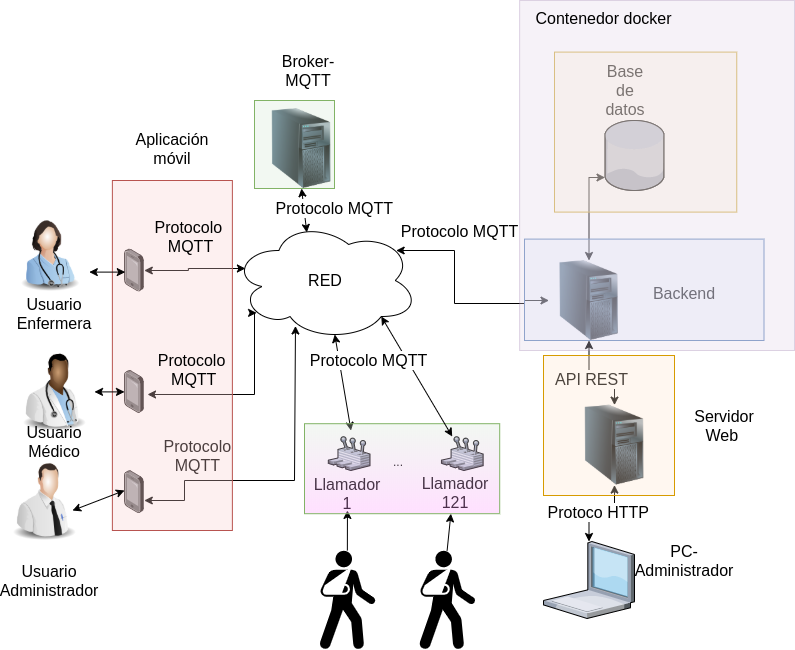
\includegraphics[scale=.45]{./Figures/DiagramaSistemaOrganizado.png}
	\caption{División del sistema.}
	\label{fig:División del sistema}
\end{figure}



\pagebreak

\section{Descripción del protocolo MQTT}
\label{sec:Descripción del protocolo MQTT}

MQTT fue introducido en 1999 por IBM y Eurotech. Es un protocolo de mensajería por suscripción/publicación especialmente diseñado para la comunicación M2M(\textit{Machine to Machine}, Máquina a Máquina) en dispositivos con bajos recursos \citep{WEBSITE:5} .

Para poder explicar el funcionamiento del protocolo es necesario incorporar conceptos definidos en la especificación \citep{WEBSITE:5}:

\begin{itemize}
\item Mensaje: datos transmitidos mediante el protocolo MQTT  a través de la red por la aplicación. Cuando un mensaje es transmitido, el mismo contiene datos útiles(\textit{"payload"}), un campo que identifica la Calidad de Servicio (\textit{Quality of Service}, QoS), ciertas propiedades y un nombre de tópico.
\item Cliente: programa o dispositivo que utiliza MQTT.
\item Servidor o Broker: programa o dispositivo que actúa como intermediario entre clientes que publican mensajes y clientes que han realizado suscripciones.
\item Sesión: una interacción entre cliente y servidor con estados bien definidos.
\item suscripción: una  suscripción implica un filtrado de tópicos y una máxima calidad de servicio. Una suscripción está asociada a una sola sesión y una sesión puede poseer varias suscripciones.
\item Nombre de tópico: etiqueta que se adjunta a un mensaje la cual es comparada con las suscripciones conocidas en el servidor.
\item Filtro de tópico: es una expresión contenida dentro de la suscripción para indicar interés, por parte del cliente, en uno o más tópicos.
\item Suscripción con comodín o \textit{Wildcard} : es una expresión contenida dentro de la suscripción que contiene un carácter especial o comodín, como ser '+' o '\# ', que representan un nivel único y nivel múltiple respectivamente.

\end{itemize}

En este protocolo, el funcionamiento es el siguiente: 

Al iniciar la conexión, el cliente envía un mensaje CONNECT al broker y este contesta con un CONNECTACK y un código de estado. El broker mantiene abierta la conexión hasta que el cliente envía un comando de desconexión o la conexión se pierde por algún motivo. Los puertos estándar son 1883 para comunicación no encriptada y 8883 para comunicación encriptada utilizando TLS/SSL \citep{ARTICLE:4}.

Luego el cliente MQTT publica mensajes en un broker MQTT, los cuales son recibidos por los clientes suscriptos o bien retenidos para una futura suscripción \citep{WEBSITE:5}. En la figura \ref{fig:Sistema MQTT} se presentan todos los componentes de una red MQTT:  

\begin{figure}[ht]
	\centering
	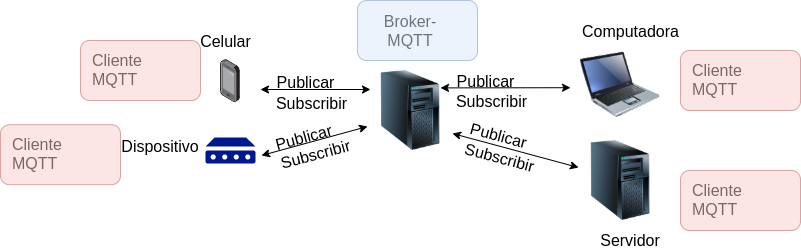
\includegraphics[scale=.45]{./Figures/MQTT-minimal.png}
	\caption{Esquema de un sistema MQTT.}
	\label{fig:Sistema MQTT}
\end{figure}

La conexión MQTT siempre es entre cliente y broker, nunca entre clientes directamente.


Cada mensaje es publicado en una dirección conocida como "tópico". Los clientes pueden subscribirse a múltiples tópicos y recibir todos los mensajes publicados en cada tópico. MQTT es un protocolo binario y normalmente requiere un encabezado fijo de dos \textit{bytes} y un dato útil (\textit{"payload"}) de hasta 256 MB \citep{ARTICLE:2} . 

Ejemplos de tópicos:

\begin{itemize}
\item  1: /user/1/question
\item  2: /user/1/\#
\item  3: /user/+/question
%\item Capítulo 2: Introducción específica
%\item Capítulo 3: Diseño e implementación
%\item Capítulo 4: Ensayos y resultados
%\item Capítulo 5: Conclusiones
\end{itemize}

En el ejemplo 1, en caso de suscribirse a ese tópico, el cliente recibirá todos los mensajes publicados en el subtópico "question".
En el ejemplo 2, el cliente recibirá todos los mensajes dirigidos al usuario 1.
En el ejemplo 3, el cliente que se suscriba a ese tópico recibirá los mensajes enviados a "question" independientemente del número de usuario.


Utiliza usualmente TCP/IP como protocolo de transporte y puede implementar TLS/SLL para seguridad. Por lo que el servicio cliente-broker es del tipo orientado a la conexión. También puede utilizar otros protocolos de red con soporte bidireccional y sin pérdidas de datos \citep{ARTICLE:4} \citep{WEBSITE:5} .


Por otro lado, el protocolo posee tres niveles de calidad de servicio ("QoS", del ingles \textit{Quality of Service}) que permite seleccionar la fiabilidad de la entrega de los mensajes \citep{WEBSITE:5}\citep{WEBSITE:28} :

\begin{itemize}
\item Calidad 0: el mensaje se entrega como máximo una vez, sino no se entrega. Es el modo mas rápido de entrega.
\item Calidad 1: el mensaje se entrega como mínimo una vez. El mensaje se almacena localmente en el emisor y el receptor hasta que se procese. Si no se confirma la recepción se envía de nuevo con el distintivo ''DUP'' establecido hasta que se reciba acuse de recibo.
\item Calidad 2: el mensaje se entrega exactamente una sola vez. El mensaje se almacena localmente en el emisor y el receptor hasta que se procese. El emisor recibe un mensaje acuse de recibo. Si el emisor no recibe un acuse de recibo, el mensaje se envía de nuevo con el distintivo DUP establecido hasta que se reciba un acuse de recibo.
En el segundo par de transmisiones, el remitente indica al destinatario que puede completar el proceso del mensaje, ''PUBREL''. Si el remitente no recibe un acuse de recibo del mensaje ''PUBREL'', el ''PUBREL'' se envía de nuevo hasta que se recibe un acuse de recibo. El remitente suprime el mensaje que ha guardado cuando recibe el acuse de recibo al mensaje “PUBREL” .

El receptor puede procesar el mensaje proporcionado en la primera o segunda fase, no tiene que volver a procesarlo. Si el receptor es un intermediario, publica el mensaje a los suscriptores. Si el receptor es un cliente, el mensaje se entrega a la aplicación de suscriptor. El receptor devuelve un mensaje de finalización al emisor para comunicarle que ha terminado de procesar el mensaje.

\end{itemize}


\label{subsec:WebSockets}
\subsection{Uso de WebSockets en MQTT}

Actualmente no es posible utilizar MQTT natural en un \textit{browser} o navegador debido a la imposibilidad de abrir una conexión TCP pura. 

Una solución a este problema puede ser transmitir el mensaje MQTT sobre una conexión WebSocket lo que permite que un \textit{browser} pueda utilizar todas las características del protocolo directamente. Esto es muy útil en el caso de las aplicaciones de telefono móvil \citep{WEBSITE:6}. 


WebSocket es un protocolo de red que provee comunicación bidireccional entre un \textit{browser} y un servidor web. El protocolo fue estandarizado en 2011 y es soportado por todos los navegadores modernos. Como MQTT, el protocolo WebSocket está basado en TCP. En la figura \ref{fig:WebSockets MQTT} se muestra conceptualmente como se encapsula la información del protocolo MQTT dentro de una trama WebSocket:

\begin{figure}[ht]
	\centering
	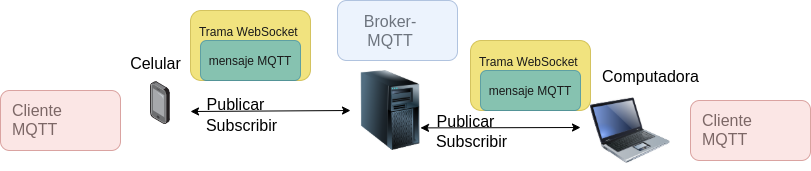
\includegraphics[scale=.45]{./Figures/websocket.png}
	\caption{Uso de WebSockets con MQTT.}
	\label{fig:WebSockets MQTT}
\end{figure}

En MQTT sobre WebSockets, el mensaje MQTT se transfiere a través de la red y es encapsulado por una o más tramas WebSockets. La ventaja de este método de transmisión es que provee una comunicación bi-direcional, ordenada y sin pérdidas \citep{WEBSITE:6} .

Para poder utilizar MQTT sobre WebSockets el Broker debe ser capaz de manejar WebSocket nativos. 

Para mejorar la seguridad, se puede implementar TLS utilizando WebSockets seguros para encriptar toda la conexión.

\label{subsec:Broker Mosquitto}
\subsection{Broker Mosquitto}

Existen muchos brokers MQTT disponibles. Para este trabajo se seleccionó Eclipse Mosquitto como Broker ya que es de código abierto con licencia EPL/EDL que implementa MQTT en sus versiones 5.0, 3.1.1 y 3.1. \citep{WEBSITE:7}.

Otra característica que lo hace muy conveniente es que se encuentra disponible en los repositorios de varias distribuciones de Linux. 




%\label{sec:ejemplo}
%\subsection{Uso de mayúscula inicial para los título de secciones}

%Si en el texto se hace alusión a diferentes partes del trabajo referirse a ellas como capítulo, sección o subsección según corresponda. Por ejemplo: ``En el capítulo \ref{Chapter1} se explica tal cosa'', o ``En la sección \ref{sec:ejemplo} se presenta lo que sea'', o ``En la subsección \ref{subsec:ejemplo} se discute otra cosa''.

%Cuando se quiere poner una lista tabulada, se hace así:

%\begin{itemize}
%	\item Este es el primer elemento de la lista.
%	\item Este es el segundo elemento de la lista.
%\end{itemize}

%Notar el uso de las mayúsculas y el punto al final de cada elemento.

%Si se desea poner una lista numerada el formato es este:

%\begin{enumerate}
%	\item Este es el primer elemento de la lista.
%	\item Este es el segundo elemento de la lista.
%\end{enumerate}

%Notar el uso de las mayúsculas y el punto al final de cada elemento.

%\subsection{Este es el título de una subsección}
%\label{subsec:ejemplo}

%Se recomienda no utilizar \textbf{texto en negritas} en ningún párrafo, %ni tampoco texto \underline{subrayado}. En cambio sí se debe utilizar %\textit{texto en itálicas} para palabras en un idioma extranjero, al menos la primera vez que aparecen en el texto. En el caso de palabras que estamos inventando se deben utilizar ``comillas'', así como también para citas textuales. Por ejemplo, un \textit{digital filter} es una especie de ``selector'' que permite separar ciertos componentes armónicos en particular.

%La escritura debe ser impersonal. Por ejemplo, no utilizar ``el diseño del firmware lo hice de acuerdo con tal principio'', sino ``el firmware fue diseñado utilizando tal principio''. 

%El trabajo es algo que al momento de escribir la memoria se supone que ya está concluido, entonces todo lo que se refiera a hacer el trabajo se narra en tiempo pasado, porque es algo que ya ocurrió. Por ejemplo, "se diseñó el firmware empleando la técnica de test driven development".

%En cambio, la memoria es algo que está vivo cada vez que el lector la lee. Por eso transcurre siempre en tiempo presente, como por ejemplo:

%''En el presente capítulo se da una visión global sobre las distintas pruebas realizadas y los resultados obtenidos. Se explica el modo en que fueron llevados a cabo los test unitarios y las pruebas del sistema''.

%Se recomienda no utilizar una sección de glosario sino colocar la descripción de las abreviaturas como parte del mismo cuerpo del texto. Por ejemplo, RTOS (\textit{Real Time Operating System}, Sistema Operativo de Tiempo Real) o en caso de considerarlo apropiado mediante notas a pie de página.

%Si se desea indicar alguna página web utilizar el siguiente formato de referencias bibliográficas, dónde las referencias se detallan en la sección de bibliografía de la memoria, utilizado el formato establecido por IEEE en \citep{IEEE:citation}. Por ejemplo, ``el presente trabajo se basa en la plataforma EDU-CIAA-NXP \citep{CIAA}, la cual...''.

%\subsection{Figuras} 

%Al insertar figuras en la memoria se deben considerar determinadas pautas. Para empezar, usar siempre tipografía claramente legible. Luego, tener claro que \textbf{es incorrecto} escribir por ejemplo esto: ``El diseño elegido es un cuadrado, como se ve en la siguiente figura:''

%\begin{figure}[h]
%\centering
%
\includegraphics[scale=.45]{./Figures/cuadradoAzul.png}
%\end{figure}

%La forma correcta de utilizar una figura es con referencias cruzadas, por ejemplo: ``Se eligió utilizar un cuadrado azul para el logo, como puede observarse en la figura \ref{fig:cuadradoAzul}''.

%\begin{figure}[ht]
%	\centering
%	
\includegraphics[scale=.45]{./Figures/cuadradoAzul.png}
%	\caption{Ilustración del cuadrado azul que se eligió para el diseño del logo.}
%	\label{fig:cuadradoAzul}
%\end{figure}

%El texto de las figuras debe estar siempre en español, excepto que se decida reproducir una figura original tomada de alguna referencia. En ese caso la referencia de la cual se tomó la figura debe ser indicada en el epígrafe de la figura e incluida como una nota al pie, como se ilustra en la figura \ref{fig:palabraIngles}.

%\begin{figure}[htpb]
%	\centering
%	
\includegraphics[scale=.3]{./Figures/word.jpeg}
%	\caption{Imagen tomada de la página oficial del procesador\protect\footnotemark.}
%	\label{fig:palabraIngles}
%\end{figure}

%\footnotetext{Imagen tomada de \url{https://goo.gl/images/i7C70w}}

%La figura y el epígrafe deben conformar una unidad cuyo significado principal pueda ser comprendido por el lector sin necesidad de leer el cuerpo central de la memoria. Para eso es necesario que el epígrafe sea todo lo detallado que corresponda y si en la figura se utilizan abreviaturas entonces aclarar su significado en el epígrafe o en la misma figura.



%\begin{figure}[ht]
%	\centering
%	
\includegraphics[scale=.37]{./Figures/questionMark.png}
%	\caption{¿Por qué de pronto aparece esta figura?}
%	\label{fig:questionMark}
%\end{figure}

%Nunca colocar una figura en el documento antes de hacer la primera referencia a ella, como se ilustra con la figura \ref{fig:questionMark}, porque sino el lector no comprenderá por qué de pronto aparece la figura en el documento, lo que distraerá su atención.

%Otra posibilidad es utilizar el entorno \textit{subfigure} para incluir más de una figura, como se puede ver en la figura \ref{fig:three graphs}. Notar que se pueden referenciar también las figuras internas individualmente de esta manera: \ref{fig:1de3}, \ref{fig:2de3} y \ref{fig:3de3}.
 
%\begin{figure}[!htpb]
%     \centering
%     \begin{subfigure}[b]{0.3\textwidth}
%         \centering
%         
\includegraphics[width=.65\textwidth]{./Figures/questionMark}
%         \caption{Un caption.}
%         \label{fig:1de3}
%     \end{subfigure}
%     \hfill
%     \begin{subfigure}[b]{0.3\textwidth}
%         \centering
%         
\includegraphics[width=.65\textwidth]{./Figures/questionMark}
%         \caption{Otro.}
%         \label{fig:2de3}
%     \end{subfigure}
%     \hfill
%     \begin{subfigure}[b]{0.3\textwidth}
%         \centering
%         
\includegraphics[width=.65\textwidth]{./Figures/questionMark}
%         \caption{Y otro más.}
%         \label{fig:3de3}
%     \end{subfigure}
%        \caption{Tres gráficos simples}
%        \label{fig:three graphs}
%\end{figure}

%El código para generar las imágenes se encuentra disponible para su reutilización en el archivo \file{Chapter2.tex}.

%\subsection{Tablas}

%Para las tablas utilizar el mismo formato que para las figuras, sólo que el epígrafe se debe colocar arriba de la tabla, como se ilustra en la tabla \ref{tab:peces}. Observar que sólo algunas filas van con líneas visibles y notar el uso de las negritas para los encabezados.  La referencia se logra utilizando el comando \verb|\ref{<label>}| donde label debe estar definida dentro del entorno de la tabla.

%\begin{verbatim}
%\begin{table}[h]
%	\centering
%	\caption[caption corto]{caption largo más descriptivo}
%	\begin{tabular}{l c c}    
%		\toprule
%		\textbf{Especie}     & \textbf{Tamaño} & \textbf{Valor}\\
%		\midrule
%		Amphiprion Ocellaris & 10 cm           & \$ 6.000 \\		
%		Hepatus Blue Tang    & 15 cm           & \$ 7.000 \\
%		Zebrasoma Xanthurus  & 12 cm           & \$ 6.800 \\
%		\bottomrule
%		\hline
%	\end{tabular}
%	\label{tab:peces}
%\end{table}
%\end{verbatim}


%\begin{table}[h]
%	\centering
%	\caption[caption corto]{caption largo más descriptivo}
%	\begin{tabular}{l c c}    
%		\toprule
%		\textbf{Especie} 	 & \textbf{Tamaño} 		& \textbf{Valor}  \\
%		\midrule
%		Amphiprion Ocellaris & 10 cm 				& \$ 6.000 \\		
%		Hepatus Blue Tang	 & 15 cm				& \$ 7.000 \\
%		Zebrasoma Xanthurus	 & 12 cm				& \$ 6.800 \\
%		\bottomrule
%		\hline
%	\end{tabular}
%	\label{tab:peces}
%\end{table}

%En cada capítulo se debe reiniciar el número de conteo de las figuras y las tablas, por ejemplo, figura 2.1 o tabla 2.1, pero no se debe reiniciar el conteo en cada sección. Por suerte la plantilla se encarga de esto por nosotros.

%\subsection{Ecuaciones}
%\label{sec:Ecuaciones}

%Al insertar ecuaciones en la memoria dentro de un entorno \textit{equation}, éstas se numeran en forma automática  y se pueden referir al igual que como se hace con las figuras y tablas, por ejemplo ver la ecuación \ref{eq:metric}.

%\begin{equation}
%	\label{eq:metric}
%	ds^2 = c^2 dt^2 \left( \frac{d\sigma^2}{1-k\sigma^2} + \sigma^2\left[ d\theta^2 + \sin^2\theta d\phi^2 \right] \right)
%\end{equation}
                                                        
%Es importante tener presente que si bien las ecuaciones pueden ser referidas por su número, también es correcto utilizar los dos puntos, como por ejemplo ``la expresión matemática que describe este comportamiento es la siguiente:''

%\begin{equation}
%	\label{eq:schrodinger}
%	\frac{\hbar^2}{2m}\nabla^2\Psi + V(\mathbf{r})\Psi = -i\hbar %%\frac{\partial\Psi}{\partial t}
%\end{equation}

%Para generar la ecuación \ref{eq:metric} se utilizó el siguiente código:

%\begin{verbatim}
%\begin{equation}
%	\label{eq:metric}
%	ds^2 = c^2 dt^2 \left( \frac{d\sigma^2}{1-k\sigma^2} + 
%	\sigma^2\left[ d\theta^2 + 
%	\sin^2\theta d\phi^2 \right] \right)
%\end{equation}
%\end{verbatim}

%Y para la ecuación \ref{eq:schrodinger}:

%\begin{verbatim}
%\begin{equation}
%	\label{eq:schrodinger}
%	\frac{\hbar^2}{2m}\nabla^2\Psi + V(\mathbf{r})\Psi = 
%	-i\hbar \frac{\partial\Psi}{\partial t}
%\end{equation}

%\end{verbatim}

\section{Descripción del protocolo HTTP}
\label{sec:Descripción del protocolo HTTP}

HTTP es un protocolo que nos permite realizar una petición de datos y recursos como ser documentos HTML que pueden mostrarse en navegadores. Es la base de cualquier intercambio en la red \citep{WEBSITE:19}. En la figura \ref{fig:Protocolo HTTP } se observa donde se ubica el protocolo dentro del modelo de comunicación TCP/IP :


\begin{figure}[ht]
	\centering
	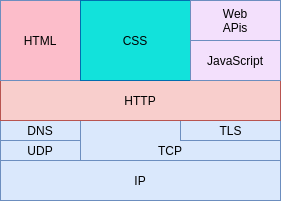
\includegraphics[scale=.5]{./Figures/http.png}
	\caption{Pila de comunicaciones en un navegador.}
	\label{fig:Protocolo HTTP }
\end{figure}

HTTP se basa en el modelo cliente-servidor: las peticiones son enviadas por una entidad al servidor, el cual gestiona y responde.

Entre las características principales figuran \citep{WEBSITE:19}:
\begin{itemize}
\item Es sencillo.
\item Puede expandirse.
\item Es un protocolo de sesiones pero no de estados: no guarda ningún dato entre dos peticiones en la misma sesión.
\item Las conexiones se realizan en la capa de transporte por lo que quedan fuera del protocolo HTTP.
\end{itemize}

La secuencia de la comunicación entre el cliente y el servidor es la siguiente \citep{WEBSITE:19}:
\begin{enumerate}
\item Se abre conexión TCP: la conexión TCP se utiliza para hacer una petición, o varias, y recibir la respuesta. El cliente puede abrir una conexión nueva, reusar la existente o abrir varias a la vez hacia el servidor.
\item Hacer una peticion HTTP: los mensajes HTTP son legibles en texto plano.
\item Se lee la respuesta enviada por el servidor.
\item Se cierra o reusa la conexión.
\end{enumerate}

En el encabezado del mensaje HTTP se puede introducir información de la sesión. Lo cual resulta muy importante en referencia a la seguridad. 


\section{Sistemas de contenedores Docker}
\label{sec:Docker}

Desde los origenes de la programación, existió una necesidad de abstraer la aplicación desarrollada de la plataforma en la que se ejecuta. Múltiples avances se fueron dando desde ese entonces: sistemas operativos con interfaces de aplicaciones estandar, librerías portables y lenguajes interpretados en máquinas virtuales son algunos de ellos.

Docker es un proyecto de código abierto que permite automatizar el despliegue de aplicaciones dentro de contenedores de software proporcionando una capa de abstracción y automatización. Fue desarrollado por Docker Inc. y su primera versión fue liberada en 2013. Está escrito en el lenguaje Golang y actualmente es un estandar en la industria del Software \citep{WEBSITE:8}.



\begin{figure}[ht]
	\centering
	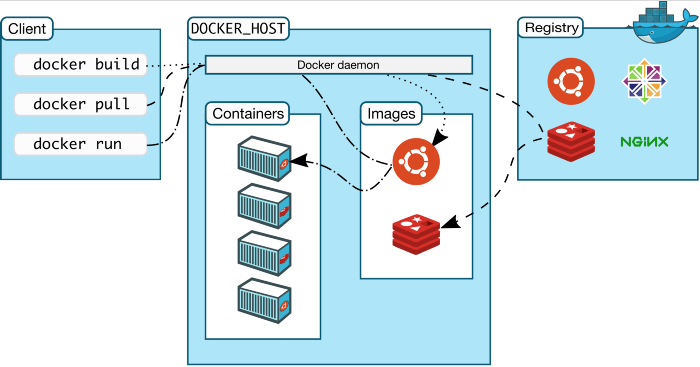
\includegraphics[scale=.5]{./Figures/docker.png}
	\caption{Estructura general de Docker.\protect\footnotemark.}
	\label{fig:Contenedores Docker. }

\end{figure}
\footnotetext{Imagen tomada de \citep{WEBSITE:8}}


Un contenedor de software es un componente aislado que se ejecuta como un proceso mas dentro del sistema operativo del host y posee todas las dependencias y requerimientos que la aplicación necesita para funcionar correctamente. Por cada contenedor en ejecución hay un proceso ejecutandose en el sistema \citep{WEBSITE:8}.

Las partes que componen del ecosistema Docker pueden resumirse de la siguiente manera \citep{WEBSITE:8}\citep{WEBSITE:9}:

\begin{itemize}
\item \textit{Images}: son plantillas que describen el contenedor. Se componen de una base y sobre estas se modifica según necesidad.
\item \textit{Containers}: son instancias de ejecución de una imagen. Se pueden iniciar, detener, mover o eliminar mediante comandos. Se puede conectar un contenedor a una o mas redes.
\item \textit{Networks}: Docker utiliza una interfaz virtual para comunicarse con la red del equipo host.
\item \textit{Volumes}: permiten generar espacios de almacenamiento dentro de cada contenedor, el funcionamiento es similar a las carpetas compartidas en las máquinas virtuales.
\item \textit{Registry}: un registro almacena imágenes de docker. Dockerhub es un registro público que cualquiera puede utilizar.
\end{itemize}

Para poder correr un contenedor docker es necesario ejecutar el comando:
\begin{lstlisting}[label=docker:vControl,caption=Ejecución de contenedor.]  
>docker-run --[parametro1] --[parametro2] ...
nombre_contendor:version
\end{lstlisting}


\subsection{Uso de Docker-compose}
\label{subsec:Docker-compose}

Docker Compose es una herramienta del ecosistema Docker que sirve para definir aplicaciones multicontenedor. La configuración se guarda en un archivo de texto llamado "docker-compose.yml". 
Con esta herramienta se facilita el paso de parámetros al contenedor y posibilita generar imágenes complejas utilizando e interconectando distintos contenedores.

 

\section{Introducción a las bases de datos}
\label{sec: Introducción a las bases de datos}

Se define un dato como un elemento o característica que permite hacer la descripción de un objeto \citep{WEBSITE:12}. En el contexto de los sistemas de Internet de las Cosas, es la mínima expresión de información que se puede gestionar.

Una base de datos es una colección de datos (o información) organizados, estructurados y almacenados electrónicamente en un sistema de computadoras. En su mayoría son controladas por un DBMS (\textit{database management system}, sistema gestor de bases de datos). Los datos, el DBMS y la aplicación que está asociada a ellos, conforman el llamado sistema de base de datos, o base de datos en forma abreviada \citep{WEBSITE:11}.

Durante los años 80 se popularizó el tipo de base de dato relacional, cuya información se organizaba como un conjunto de tablas con columnas y filas. Este tipo de base de datos provee la forma más eficiente y flexible de acceder a información estructurada.

En 1970, IBM junto a Oracle desarrollaron un lenguaje de programación llamado SQL (\textit{Structured Query Language}, Lenguaje de Colas Estructurado). Su principal objetivo era manipular, encolar, definir datos y proveer control de acceso en las bases de datos relacionales. Este lenguaje es apliamente utilizado hoy en día, aún cuando surgen nuevos.

Se podría empezar a clasificar las bases de datos en relacionales y no relacionales. Las primeras utilizan SQL como su lenguaje de programación y entre ellas podemos encontrar: PostgreSQL, MySQL y SQL Server. Las segundas no utilizan un lenguaje SQL, ya que no trabajan en base a estructuras definidas, poseen una gran escalabilidad y estan diseñadas para manejar grandes volumentes de datos \citep{WEBSITE:12}.


\subsection{Descripción de MySQL}
\label{subsec: Bases de datos relacionales}

En este trabajo se seleccionó el DBMS MySQL. Es un sistema de gestión de bases de datos con mas de 10 millones de instalaciones. Fue desarrollado a mediados de la década de los 90, y es de uso libre. Es potente, rápido y altamente escalable \citep{BOOK:2}.

Existen tres formas de interactuar con una base de datos MySQL: utilizando la consola, a través de una interfaz web como phpMyAdmin y mediante un lenguaje de programación.

En la figura \ref{fig:Página phpMyAdmin} se puede observar la interfaz:

 
\begin{figure}[ht]
	\centering
	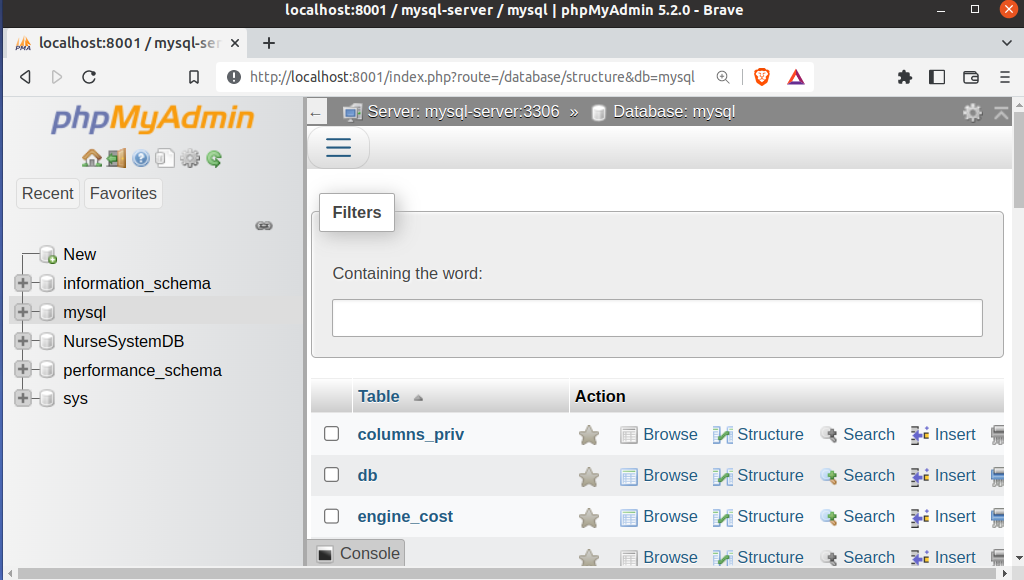
\includegraphics[scale=.35]{./Figures/phpMyAdmin.png}
	\caption{Página de gestión phpMyAdmin.}
	\label{fig:Página phpMyAdmin}
\end{figure}

Los comandos más utilizados en SQL se observan en la tabla \ref{tab:Funciones SQL} \citep{BOOK:2}:

%\begin{verbatim}
\begin{table}[h]
	\centering
	\caption[Comandos SQL]{Comandos básicos SQL.}
	\begin{tabular}{l c }    
		\toprule
		\textbf{Comando}     & \textbf{Función} \\
		\midrule
		ALTER & Modificar una base de datos o una tabla    \\		
		BACKUP    & Copia de seguridad de una tabla      \\
		$\backslash$c  & Cancelar la entrada\\
		CREATE  & Crear la base de datos\\
		DELETE  & Borrar una fila de una tabla\\
		DESCRIBE  & Describir columnas de una tabla\\
		DROP  & Eliminar una base de datos o una tabla\\
		EXIT & Salir.\\
		GRANT & Cambiar permisos de un usuario\\
		INSERT INTO..VALUES & Insertar datos\\
		RENAME & Cambiar nombre de una tabla\\
		USE & Usar una base de datos\\
		UPDATE & Actualizar un registro existente\\
		SELECT  & Consultar una fila\\
		JOIN... ON & Consultar múltiples tablas\\
		\bottomrule
		\hline
	\end{tabular}
	\label{tab:Funciones SQL}
\end{table}
\pagebreak
Ejemplo de uso, suponiendo 2 tablas:

\begin{table}[h]
	\centering
	\caption[Tabla 1 Ejemplo SQL]{TABLA1 para el ejemplo 1.}
	\begin{tabular}{l c c}    
		\toprule
		\textbf{PacienteId}     & \textbf{Nombre} \\
		\midrule
		 1& Pedro    \\		
 		 2& Juan    \\				
		\bottomrule
		\hline
	\end{tabular}
	\label{tab:Ejemplo 1}
\end{table}

\begin{table}[h]
	\centering
	\caption[Tabla 2 Ejemplo SQL]{TABLA2 para el ejemplo 1.}
	\begin{tabular}{l c c}    
		\toprule
		\textbf{PacienteId}     & \textbf{Apellido} \\
		\midrule
		 1& Perez    \\		
 		 2& Salvador    \\	
		\bottomrule
		\hline
	\end{tabular}
	\label{tab:Ejemplo 2}
\end{table}

Si se quiere obtener el nombre y apellido del paciente con pacienteId igual a 1, una forma de obternerlo es ejecutando el código:

\begin{lstlisting}[label=código:SQL:vControl,caption=Ejecución de comando sql]  
>SELECT Nombre,Apellido FROM TABLA1 as TB1 \
JOIN TABLA2 as TB2 ON TB1.pacienteId=TB2.pacienteId \
WHERE TB1.pacienteId=1;
>Pedro Perez
\end{lstlisting}

Una de las múltiples ventajas que poseen los motores de bases de datos relacionales es la posibilidad de realizar transacciones. Las mismas consisten en secuencias de operaciones que se ejecutan en orden y se completan con éxito.

\begin{lstlisting}[label=código:SQL2:vControl,caption=Secuencia de transacción SQL.]  
>BEGIN;
>SELECT Nombre FROM  TABLA1;
>SELECT Apellido FROM  TABLA2;
>COMMIT;
>Pedro 
>Juan
>Perez
>Salvador
\end{lstlisting}


\section{Frameworks/librerías para desarrollo web/móvil}

En esta sección se presentan las librerías y frameworks que se utilizaron para el desarrollo.

\subsection{Librerías Node.js, Express y JWT}
\label{subsec: Node}
El trabajo realizado utiliza como lenguaje de programación  Javascript para las tareas del backend. Para generar el servidor se utiliza Node.js \citep{WEBSITE:20}, que es un \textit{runtime environment}(entorno de ejecución) de Javascript. Node.js se encuentra orientado a eventos asíncronos y está diseñado para crear aplicaciones de red escalables.

Ademas de la alta velocidad de ejecución, Node.js posee un bucle de eventos (\textit{Event loop}), que permite gestionar múltiples clientes de forma asíncrona. La principal ventaja que posee el método de bucle de eventos de Node.js con respecto al método tradicional (que se valían de programación basada en hilos) es que no escala la cantidad de memoria a utilizar a medida de que se aumentan las conexiones.

Por ultimo, es importante mecionar que Node.js posee un gestor de paquetes/librerías llamado NPM, que permite fácilmente incorporar piezas de software probadas a los proyectos.


Para el ruteo de los endpoints con los que se comunica la página web se utiliza Express.js \citep{WEBSITE:21} que es una infraestructura web rápida, minimalista y flexible para Node.js. 

Express.js facilita la creación de la API(\textit{Application Program Interface}, Interfaz de Programación de Aplicaciones), asi como la incorporación de software \textit{Middleware}. 

Con respecto a la seguridad para el acceso de la página web, existen dos métodos: por medio de \textit{cookies} o por medio de web \textit{tokens}. Se seleccionó utilizar el segundo y para ello se utiliza JWT \citep{WEBSITE:22} que implementa el estandar RFC 7519. 



\subsection{Framework Ionic/Angular, Capacitor y Android Studio}
\label{subsec: Ionic}

Drifty.co introdujo Ionic en el año 2013 \citep{WEBSITE:24}. Nació originalmente para desarrollar aplicaciones móviles con Angular 1 pero hoy en día permite desarrollar para dispositivos celulares, páginas web progresivas y aplicaciones de escritorio junto con Electron \citep{WEBSITE:25}. Ionic permite trabajar con Vue, React y Angular en su última versión.

Este framework posee muchos \textit{plugins}(o software de ayuda) que permiten acceder a los recursos de los dispositivos móviles como ser su micrófono, la cámara, la información de posicionamiento, entre otros. Junto con Ionic se utiliza Capacitor \citep{WEBSITE:26}, que es un runtime nativo para iOS, Android y aplicaciones web progresivas.

El código que genera Ionic debe compilarse para generar el archivo ejecutable(ya sea .ipa para iOS o .apk para Android). Para ello, se utilizan los entornos de desarrollo Xcode para iOS, y Android Studio para Android.

Por ejemplo, el método de desarrollo para una aplicación que se ejecutará en un dispositivo Android es el siguiente:

\begin{enumerate}
\item Desarrollo: se genera el código fuente en una pc.
\item Prueba virtual en el navegador:  se realiza debug localmente, utilizando los comandos ionic serve o ionic-lab
\item Prueba en el disposito: se genera un \textit{build}(construcción de software) y se carga Android Studio. Luego se descarga en el dispositivo.
\end{enumerate}
